\documentclass[ngerman,11pt]{article}

\usepackage[utf8]{fontenc}
\usepackage[left=1.5cm, right=1.5cm, top=1cm, bottom=1cm]{geometry}
\usepackage{babel}
\usepackage{listings}
\usepackage{color}
\usepackage{hyperref}
\usepackage{csquotes}
\usepackage{awesomebox}
\usepackage{multicol}
\MakeOuterQuote{"}

\definecolor{dkgreen}{rgb}{0,0.6,0}
\definecolor{gray}{rgb}{0.5,0.5,0.5}
\definecolor{mauve}{rgb}{0.58,0,0.82}


\pagenumbering{gobble}
\renewcommand{\lstlistingname}{Schnipsel}

\lstset{frame=tb,
    language=Python,
    aboveskip=3mm,
    belowskip=3mm,
    showstringspaces=false,
    captionpos=b,
    columns=flexible,
    basicstyle={\small\ttfamily},
    numbers=left,
    numberstyle=\tiny\color{gray},
    keywordstyle=\color{blue},
    commentstyle=\color{dkgreen},
    stringstyle=\color{mauve},
    breaklines=true,
    breakatwhitespace=true,
    tabsize=3,
    inputencoding=utf8
}

% Packages
\usepackage{amsmath}
\usepackage{graphicx}

% Document
\begin{document}

    \setlength{\parindent}{0}

    {\huge \textbf{Programmieren mit Python und Turtle}}

    \vspace{1cm}


    \section{Zusammenfassung / Wiederholung}

    Wir haben in den letzten Wochen die Grundlagen der Programmierung mit Python kennengelernt.
    Dazu verwendeten wir die "Schildkröte" in Python-Turtle welche wir mit bestimmten
    Befehlen bewegen können, um Linien auf dem Bildschirm zu zeichnen. \\

    \subsection{Grundlagen}

    Ein einfaches Turtle-Programm sieht zum Beispiel so aus: \\

    \begin{lstlisting}[caption=Simples Muster,label={lst:p1}]
from turtle import *

# Bewegt die Schildkroete um 100 Einheiten nach vorne
forward(100)

# Dreht die Schildkroete um 90 Grad nach rechts
right(90)

forward(100)
right(90)
forward(100)
right(90)
forward(100)
right(90)

# Sorgt dafuer, dass das Fenster am Ende nicht sofort verschwindet
mainloop()
    \end{lstlisting}

    \textbf{Aufgabe 1}: Kannst du sagen, was das Programm in Schnipsel~\ref{lst:p1} tut, ohne es auszuführen? \\

    \textbf{Aufgabe 2}: Schreibe ein Programm, welches die Schildkröte den Buchstaben \lstinline{A} zeichnen lässt. \\

    Das erste Konzept der Programmierung, welches wir kennengelernt haben, ist die Verwendung
    von \textit{Variablen}.
    Jede Variable hat einen \texit{Namen} und einen \textit{Wert}.
    Die beiden wichtigsten Vorteile von Variablen sind, dass unser Programmcode
    \begin{itemize}
        \item besser verständlich
        \item einfacher zu ändern
    \end{itemize}
    wird. \\

    Beispiel:

    \begin{lstlisting}[caption=gleichseitiges Dreieck,label={last:p2}]
from turtle import *

right(120)
forward(100)
right(120)
forward(100)
right(120)
forward(100)

mainloop()
    \end{lstlisting}

    Was tut dieses Programm?
    Wenn wir uns das Programm genau anschauen, sehen wir, dass 3 Drehungen mit anschließender
    Bewegung nach vorne geschehen, und somit ein gleichseitiges Dreieck gezeichnet wird.
    Um darauf zu kommen, müssen wir uns jede einzelne Zeile des Programms genau durchlesen. \\

    \subsection{Variablen}

    Vergleichen wir das Programm mit dieser Version:

    \begin{lstlisting}[caption=gleichseitiges Dreieck mit Variable,label={last:p3}]
from turtle import *

seitenlaenge = 100

right(120)
forward(seitenlaenge)
right(120)
forward(seitenlaenge)
right(120)
forward(seitenlaenge)

mainloop()
    \end{lstlisting}

    Jetzt ist viel klarer, was die \lstinline{100} in unserem Programm bedeutet
    und auf einen Blick ersichtlich, dass 3 gleich lange Linien gezeichnet werden. \\

    Allgemein werden Variablen in Python also wie folgt definiert:

    \begin{lstlisting}
[name] = [wert]
    \end{lstlisting}

    wobei wir \lstinline{[name]} mit dem Namen der Variable ersetzen und \lstinline{[wert]} mit dem Wert.
    Variablen können wir dann überall dort verwenden, wo wir den Wert direkt verwenden könnten. \\

    Beispiele:

    \begin{lstlisting}[caption=Variablen]
seitenlaenge = 350
forward(seitenlaenge)

winkel = 110
right(110)

name = "Mareike"
print(name)
    \end{lstlisting}

    \textbf{Aufgabe 3}: Schreibe ein Programm, welches ein Rechteck zeichnet.
    Die Höhe und die Breite des Rechtecks sollen dabei über jeweils eine eigene Variable änderbar sein.

    \newpage

    \subsection{Schleifen}

    Oft ist es so, dass wir für die Lösung eines Problems (also die Umsetzung eines Algorithmus)
    Schritte wiederholen müssen. \\

    Beispiel: Ein Algorithmus, der beschreibt wie man "einmal um den Block fährt",
    könnte wie folgt aussehen: \\

    {\color{red}\verb_Algorithmus: BLOCK (1)_} \\
    \verb_Fahre gerade aus bis zur nächsten Kreuzung_ \\
    \verb_Biege nach rechts ab_ \\
    \verb_Fahre gerade aus bis zur nächsten Kreuzung_ \\
    \verb_Biege nach rechts ab_ \\
    \verb_Fahre gerade aus bis zur nächsten Kreuzung_ \\
    \verb_Biege nach rechts ab_ \\
    \verb_Fahre gerade aus bis zur nächsten Kreuzung_ \\
    \verb_Biege nach rechts ab_ \\

    Natürlich könnten wir diesen Algorithmus wie folgt abkürzen: \\

    {\color{red}\verb_Algorithmus: BLOCK (2)_} \\
    \verb_[Tue die folgenden Dinge 4 mal]_ \\
    \verb_| Fahre gerade aus bis zur nächsten Kreuzung_ \\
    \verb_| Biege nach rechts ab_ \\

    \notebox{
        Dieser Algorithmus ist nicht korrekt (das heißt, er führt nicht immer zum richtigen Ergebnis), siehst du wieso?
        Kannst du ihn korrigieren?
    }

    Genau das gleiche können wir in Python mithilfe von Schleifen tun.
    Der Vorteil ist, dass wir uns nicht so oft wiederholen und wieder viel
    genauer sagen können was wir tun wollen.
    (Die Anweisung \textit{"Mache 4 mal diese 2 Dinge: \dots"} ist wesentlich klarer als \textit{"Mache diese 8 Dinge: \dots"})

    Schauen wir noch einmal auf das Beispiel aus Schnipsel~\ref{lst:p1}:

    \begin{lstlisting}[caption=Rechteck]
forward(100)
right(90)
forward(100)
right(90)
forward(100)
right(90)
forward(100)
right(90)
    \end{lstlisting}

    Schauen wir genau hin, sehen wir dass die ersten beiden Zeilen vier mal wiederholt werden.
    In Python notieren wir das wie folgt:

    \begin{lstlisting}[caption=Rechteck mit Schleife]
for i in range(0, 4):
    forward(100)
    right(90)
    \end{lstlisting}

    Das hat diese Bedeutung:
    \lstinline{range(0, 4)} konstruiert ein Folge von Zahlen: \lstinline{0, 1, 2, 3}.
    Für jede dieser Zahlen wird der eingerückte Code "in" der for-schleife je einmal ausgeführt.

    \tipbox{
        "Einrücken" bedeutet den Code nach rechts zu verschieben.
        Die Verschiebung muss in Python immer gleich sein (also zum Beispiel 0 Leerzeichen ganz links, 4 Leerzeichen auf der nächsten Ebene, und so weiter), sonst
        kann es zu Fehlern kommen.
        Am einfachsten geht es, wenn man mehrere Zeilen auswählt und dann "Tabulator" (Doppelpfeil) drückt.
    }

    \notebox{Bei {\verb_range(a, b)} ist die Linke Zahl enthalten, die rechte aber nicht.
Eine Schleife der Form {\verb_range(1, 5)} läuft also zum Beispiel 4 mal, nicht 5 mal.}

    \vspace{1cm}

    \textbf{Aufgabe 4}: Schreibe ein Programm, welches ein reguläres 8-Eck zeichnet.
    Verwende dazu nicht mehr als 3 Zeilen Code (abgesehen von \lstinline{from turtle import *} und \lstinline{mainloop()}).

    \tipbox{
        \textbf{Tipp}: Ein reguläres n-Eck hat eine Innenwinkelsumme von $(n - 2) \cdot 180$ Grad.
        Für ein 8-Eck ergibt sich damit 1080 Grad.
        Jeder einzelne Innenwinkel beträgt also $\frac{1080}{8} = 135$ Grad.
        Um wie viel Grad muss sich die Schildkroete nun drehen, um einen Innenwinkel von 135 Grad zu erzeugen?
    }

    \newpage


    \section{Weiterführende Befehle}

    \subsection{Gestaltung}

    Wir wollen uns ein paar Möglichkeiten ansehen, wie wird das Erscheinungsbild
    der Turtle-Zeichnung anpassen können. \\

    Vorab: Haben wir ein langes Programm, sodass wir zu lange zuschauen müssen wie gezeichnet wird,
    können wir die Geschwindigkeit ändern.
    Das geht mit der Funktion \verb_speed_.
    Wir suchen uns einfach die für unsere Situation passende Geschwindigkeit aus:

    \begin{lstlisting}[caption=Geschwindigkeit ändern]
speed("fastest")
speed("fast")
speed("normal")
speed("slow")
speed("slowest")
    \end{lstlisting}

    \textbf{Aufgabe 5}: Probiere die Folgenden Befehle nacheinander (!) aus und schau, was diese bewirken.

    \begin{lstlisting}[caption=Erscheinungsbild]
shape("turtle")
pencolor("green")
width(5)
    \end{lstlisting}

    \subsection{Weitere Bausteine}

    Wir haben bisher der Einfachheit halber fast nur die Befehle \verb_forward_ und \verb_right_
    verwendet.
    Im Folgenden eine Liste mit weiteren Befehlen, die wir verwenden können, um kompliziertere Dinge zu zeichnen.

    \begin{lstlisting}[Turtle Befehle - Übersich]
# Bringt die Schildkroete "nach Hause" (also zu den Koordinaten (0, 0))
home()

# Hebt den Stift an, die Kroete hört also auf zu zeichnen wenn sie sich bewegt
penup()

# Senkt den Stift wieder, sodass wieder gezeichnet wird
pendown()

# Bewegt die Kroete vorwärts / rückwärts um die angegebene Distanz
forward(100)
backward(100)

# Dreht die Schildkroete im / gegen den Uhrzeigersinn um den angegebenen Winkel
right(80)
left(80)

# Zeichnet einen Kreis mit dem angegebenen Radius
circle(40)

# Malt einen "Punkt" mit der angegebenen Groesse und Farbe
dot(15, "blue")

# Teleportiert die Schildkroete (ohne zu zeichnen) an die angegebenen Koordinaten (x, y)
teleport(50, -30)
    \end{lstlisting}

    \newpage


    \section{Aufgaben / Inspiration}

    Im Folgenden siehst du Bilder von Turtle-Zeichnungen.
    Versuche beliebige davon wie abgebildet oder leicht angepasst nachzuprogrammieren. \\


    \begin{multicols}{2}
        
\includegraphics[width=0.45\textwidth]{german}
        
\includegraphics[width=0.45\textwidth]{thing}
        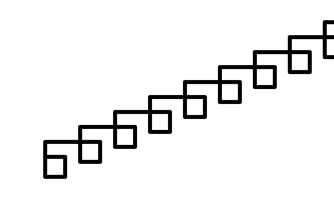
\includegraphics[width=0.45\textwidth]{spiral1}
        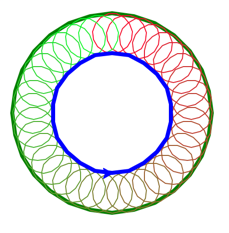
\includegraphics[width=0.45\textwidth]{round}
        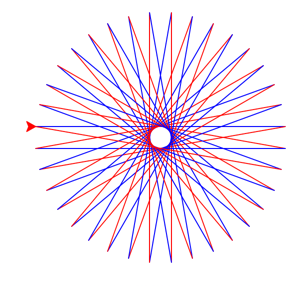
\includegraphics[width=0.45\textwidth]{star}
    \end{multicols}
\end{document}
